\documentclass{article}
    
\usepackage{Haust2017skil}
\usepackage{caption}
\usepackage{subcaption}

\title{Stærðfræðimynstur í tölvunarfræði \\ Skilaverkefni 13}
\author{}

\begin{document}
\maketitle

13. kafli bókarinnar er ekki í Global útgáfunni. Skrá sem inniheldur kaflann má nálgast á Piazza.
Skilmálar frá fyrri verkefnaskömmtum eru enn í gildi.

\section{Kafli 11.4}

\question Notið dýptarleit til að finna spanntré fyrir eftirfarandi net. Veljið $a$ sem rót. Þegar velja þarf á milli jafngildra hnúta, veljið í stafrófsröð. Gefið lausn með því að teikna tréð.

\begin{center}
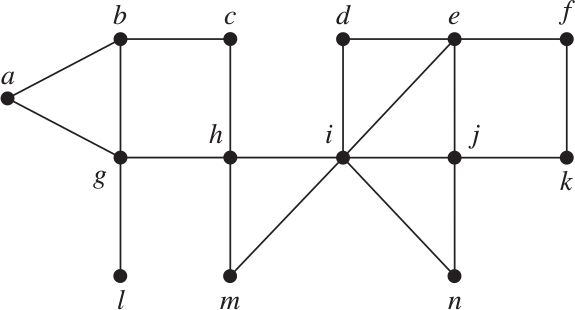
\includegraphics[width=0.45\textwidth]{tree-spanning-exercise}
\end{center}

\textbf{Í bók:} Exercise 11.4.14

\section{Kafli 11.5}

\question Finnið tvö léttustu spanntré í eftirfarandi neti, annars vegar með reikniriti Prims og hins vegar með reikniriti Kruskals. Gefið lausn með því að teikna trén.

\begin{center}
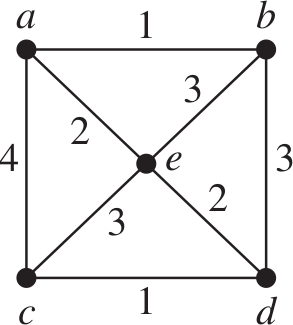
\includegraphics[width=0.2\textwidth]{tree-spanning-minimum-exercise}
\end{center}

\textbf{Í bók:} Byggt á Exercise 11.5.2

\section{Kafli 13.3}

\question Lýsið mengi strengjanna sem eftirfarandi stöðuvél samþykkir.

\begin{center}
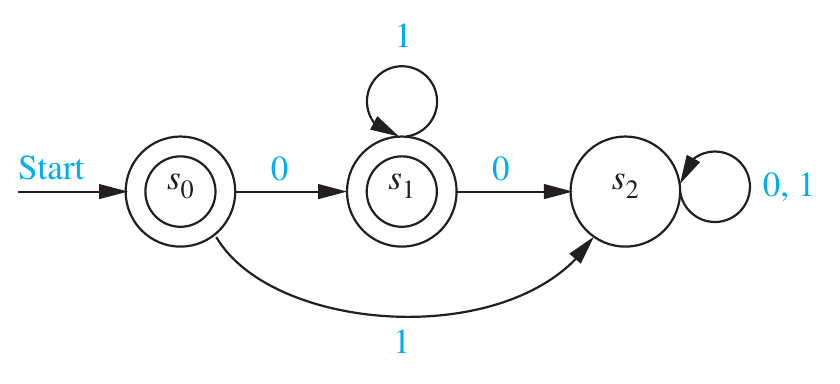
\includegraphics[width=0.5\textwidth]{dfa-exercise2}
\end{center}

\textbf{Í bók:} Exercise 13.3.18

\question Skrifið endanlegan samþykkjara (stöðuvél) sem samþykkir mengi þeirra bitastrengja sem inniheldur sléttatölufjölda af 1. Gefið lausn með því að teikna stöðuvélina.

\textbf{Í bók:} Exercise 13.3.32

\question Gefinn er brigðgengur samþykkjari. Skrifið löggengan samþykkjara sem samþykkir sama mál. Gefið lausn með því að teikna stöðuvélina.

\begin{center}
    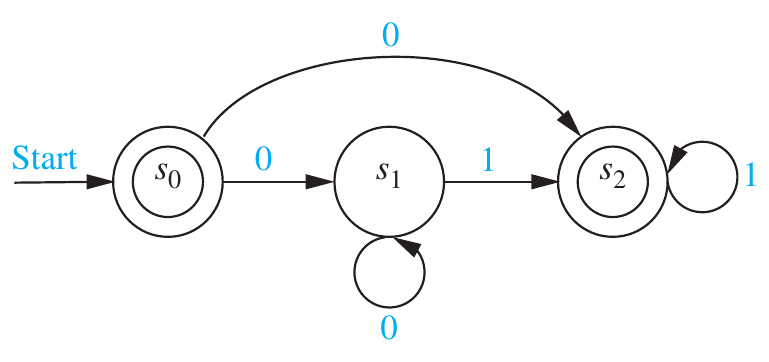
\includegraphics[width=0.5\textwidth]{nfa-exercise}
\end{center}

\textbf{Í bók:} Exercise 13.3.52

\section{Kafli 13.4}

\question Skrifið endanlegan löggengan samþykkjara sem er jafngildur reglulegu segðinni $(0 \cup 1)1^*$. Gefið lausn með því að teikna stöðuvélina.

\textbf{Í bók:} Byggt á exercise 13.4.12 b)

\end{document}
